\documentclass[a4paper,11pt,headings=standardclasses,parskip=half]{scrartcl}

% font, style, etc.
\usepackage[utf8]{inputenc} % defines
\usepackage{csquotes}
\usepackage{xspace} % proper space after macros with 0 args

% mathematics
\usepackage{amsmath}
\usepackage{amssymb}

% figures, tables, etc.
\usepackage{hyperref} %
\usepackage{graphicx}
\usepackage{tikz}
\usepackage{pgf}
\usepackage{xcolor}
\usepackage{placeins} % -> floatbarrier
\usepackage{siunitx}  % -> handling of units
\usepackage[printwatermark]{xwatermark}
\newwatermark[allpages,color=red!50,angle=45,scale=1.8,xpos=0,ypos=0]{\textsf{DRAFT ONLY, NOT APPROVED}}

% code
\usepackage{listings}
\lstset{
language=Python, 
backgroundcolor = \color{light-gray},
basicstyle=\scriptsize\sffamily,
stringstyle=\color{orange},
breaklines=true,
numberstyle=\tiny\color{gray},
keywordstyle=\bfseries\color{dark-blue}\textit, % print keywords dark-blue
commentstyle=\color{dark-green}, % print comments dark-green
showstringspaces=false} % spacing between strings not showed

\newcommand{\listcode}[3]{\lstinputlisting[numbers=left,firstnumber=#1,firstline=#1,lastline=#2]{#3}}
\newcommand{\listcodeplot}[2]{\listcode{#1}{#2}{../sim/01_car_example_plotting.py}}
\newcommand{\listcodeanim}[2]{\listcode{#1}{#2}{../sim/02_car_example_animation.py}}

% others
\usepackage{acronym}

% theorems
\newtheorem{defi}{Definition}[section]

% setup the appearance of links
\hypersetup{
    colorlinks = true, % false -> red box arround links (not very nice)
    linkcolor={blue!100!black},
    citecolor={blue!100!black},
    urlcolor={blue!100!black},
}

% manage glossaries
\usepackage{glossaries}
\makeglossaries
\newacronym{ivp}{IVP}{initial value problem}

% define shortcuts
\newcommand{\ad}{\mathrm{ad}}
\renewcommand{\d}{\mathrm{d}} % d vor differential forms
\newcommand{\NV}{{\cal N}\,}
\newcommand{\rang}{\mathrm{rang}}
\newcommand{\im}{\mathrm{im}}
\newcommand{\spann}{\mathrm{span}}
\newcommand{\R}{\mathbb{R}} %  set of real numbers
\newcommand{\py}{\emph{Python}\xspace}
\newcommand{\scipy}{\emph{SciPy}\xspace}
\newcommand{\mpl}{\emph{Matplotlib}\xspace}
\newcommand{\uu}{\mathbf{u}}
\newcommand{\x}{\mathbf{x}}
\newcommand{\y}{\mathbf{y}}
\newcommand{\z}{\mathbf{z}}
\newcommand{\xZero}{\mathbf{x}_0}

% color definitions
\definecolor{light-gray}{gray}{0.95}
\definecolor{dark-blue}{rgb}{0, 0, 0.5}
\definecolor{dark-red}{rgb}{0.5, 0, 0}
\definecolor{dark-green}{rgb}{0, 0.5, 0}
\definecolor{gray}{rgb}{0.5, 0.5, 0.5}

% ----------------------------------------------------------------------------
\subject{Control Theory Tutorial}% optional
\title{Car-Like Mobile Robot}
\subtitle{\py for simulation, animation and control}% optional
\author{}
\date{}
% ----------------------------------------------------------------------------


\begin{document}

\maketitle% create title

\tableofcontents

\newpage

\section{Introduction}
The goal of this tutorial is to teach the usage of the programming language \py as a tool for developing and simulating control systems. The following topics are covered:
\begin{itemize}
\item Implementation of the model in \py,
\item Simulation of the model,
\item Presentation of the results.
\end{itemize}
\textbf{\py source code file: \texttt{01\_car\_example\_plotting.py}}

Later in this tutorial we will extend our simulation by a visualization of the moving car and some advanced methods of numerical integration.

Please refer to the \href{http://cs231n.github.io/python-numpy-tutorial/#python-containers}{\py List-Dictionary-Tuple tutorial} and the \href{http://cs231n.github.io/python-numpy-tutorial/#numpy}{NumPy Array tutorial} if you are not familiar with the handling of containers and arrays in \py. If you are completely new to \py consult the very basic introduction on \href{https://www.tutorialspoint.com/python/index.htm}{tutorialspoint}.

\section{Model of a car-like mobile robot}
\label{sec:model}
\begin{figure}[ht]
  \centering
  \def\svgwidth{0.7\textwidth}
  \input{img/car-like_mobile_robot.pdf_tex}
  \caption{Car-like mobile robot}
  \label{fig:car}
\end{figure}
Given is a nonlinear kinematic model of a car-like mobile robot, cf.~Figure \ref{fig:car}, with the following system variables: position $(y_1, y_2)$ and orientation $\theta$ in the plane, the steering angle $\phi$ and the robots lateral velocity $v=\left| \mathbf{v} \right| $: 
\begin{subequations}\label{eq:syseq}
\begin{alignat}{2}
\dot{y}_1(t)&=v \cos (\theta(t)) &\qquad y_1(0) &= y_{10}\\
\dot{y}_2(t)&=v \sin (\theta(t)) &\qquad y_2(0) &= y_{20}\\
\tan(\phi(t)) &= \frac{l\dot{\theta}(t)}{v(t)} &\qquad \theta(0) &= \theta_{0}.
\end{alignat}
\end{subequations}
The initial values are denoted by $y_{10}$, $y_{20}$, and $\theta_0$, respectively. The velocity $v$ and the steering angle $\phi$ can be considered as an input acting on the system.

To simulate this system of 1st order ordinary differential equations (ODEs), we define a state vector $\x=(x_1,x_2,x_3)^\mathrm{T}$ and a control vector $\uu=(u_1,u_2)^\mathrm{T}$:
\begin{subequations} \label{eq:odesys}
\begin{alignat}{2}
x_1 &= y_1 &\qquad u_1 &= v\\
x_2 &= y_2 &\qquad  u_2 &= \phi \:. \\
x_3 &= \theta
\end{alignat}
\end{subequations}
Now we can express the \gls{ivp} \eqref{eq:syseq} in a general form $\dot{\x}(t)=f(\x(t),\uu(t))$, $\x(0) = \xZero$:
\label{eq:ss_system}
\begin{align}
\underbrace{\begin{pmatrix} \dot{x}_1(t) \\ \dot{x}_2(t) \\ \dot{x}_3(t) \end{pmatrix}}_{\dot{\x}(t)} = \underbrace{\begin{pmatrix}  u_1(t) \cos(x_3(t)) \\ u_1(t) \sin(x_3(t)) \\ \frac{1}{l}u_1(t) \tan(u_2(t)) \end{pmatrix}}_{f(\x(t),\uu(t))} \qquad \x(0) = \xZero.
\end{align}
This explicit formulation of the \gls{ivp} is usually the basis for implementing a numerical integration needed for simulation of the system. In the following we will setup a simulation using the programming language \py which shows how the vehicle behaves if we drive with a continously decreasing velocity under a constant steering angle (of course we know the result in advance: the car will drive on a circle until it stops for $v = 0$). We will derive the \py-script for the simulation of the system line by line.


\section{Libraries and Packages}
\py itself does not offer any functions for the direct solution of the \gls{ivp} \eqref{eq:syseq} and for the presentation of the results. Therefore, we need to import certain packages which provide utilities for the mathematical calculations, array handling, numerical integration and plotting. Under \py such packages should be imported at the top of the executed script\footnote{It is also possible to import them elsewhere in the code but this is not good style.}. The packages which are most relevant for the simulation of control systems in this tutorial are \href{http://www.numpy.org/}{NumPy} for array handling and mathematical functions, \href{https://docs.scipy.org/doc/scipy/reference/}{\scipy} for numerical integration of ordinary differential equations (and a lot of other stuff, of course) and \href{https://matplotlib.org/}{MatplotLib} for plotting.

It is good practice to connect the imported packages with a kind of namespace so we know in our code where which function comes from. In case of NumPy the following statement imports the packages NumPy and ensures that in the following every function from NumPy is addressed by the prefix \texttt{np.}:
\listcodeplot{2}{2}
For ``trivial'' functions like $\cos(\cdot), \sin(\cdot)$ and $\tan(\cdot)$ it is annoying to prefix them like \texttt{np.cos(...)} each time. To avoid this we can directly import them as 
\listcodeplot{3}{3}
To solve the \gls{ivp} \eqref{eq:ss_system} we use the library \scipy and its sub-package \emph{integrate}, which delivers different solvers for \glspl{ivp}.
\listcodeplot{4}{4}
For plotting the output of our simulation, we use the library \mpl and its sub-package \emph{pyplot}, which delivers a user experience similar to \emph{MATLAB}.
\listcodeplot{5}{5}


\section{Storing parameters}
In such simulations we usually have to deal with a lot of parameters describing the system or the simulation setup. It is a good idea to pack these parameters into one object so we do not have to deal with several individual variables holding the values of the parameters. There are several possibilities to do so. One easy way is to pack the parameters into a structure which basically is an instance of an empty class derived from \texttt{object} and susbsequently assign the members holding the parameter values:
\listcodeplot{8}{15}
The same is done with the simulation parameter:
\listcodeplot{17}{21}

Alternatively, one could use a dictionary. However, the resulting keyword notation (e.g.~\texttt{para["l"]} instead of \texttt{para.l}) in the formulas using the parameters becomes a bit annoying in that approach.


\section{Simulation with \scipy's integrate package} \label{sec:simulation}

\subsection{Implementation of the model} \label{sec:implementation-model}
To simulate \eqref{eq:ss_system} using the numerical integrators offered by \scipy's integrate package we need to implement a function which returns the right hand side of \eqref{eq:odesys} evaluated for given values of $\x$, $\uu$ and the parameters:
\listcodeplot{24}{44}
The control law calculating values for $v$ and $\phi$ depending on the state $\x$ and the time $t$ is also implemented as a function:
\listcodeplot{47}{60}
As a first simple heuristic, we drive the car with a constant steering angle and continously reduce the speed starting from \SI{0.5}{\meter\per\second} until it reaches zero. Later we can implement an arbitrary function, for expample a feedback law $\uu=k(\x)$. Note that the function needs to handle also time arrays as input in order to calculate the control for a bunch of values at once. That's why we use NumPy's array capable \href{https://docs.scipy.org/doc/numpy/reference/generated/numpy.maximum.html}{maximum function} and set the shape of \texttt{u2} appropriately.

Note the way the two functions above are documented. The text within the \texttt{"""} is called \emph{docstring}. Tools like \href{http://www.sphinx-doc.org/en/stable/}{Sphinx} are able to build well formatted documentations out of them. There are several ways the docstrings can be written in the source code files. Here we use the so-called \href{https://sphinxcontrib-napoleon.readthedocs.io/en/latest/example_google.html}{Google Style}.

\subsection{Solution of the \gls{ivp} using \scipy}
We are now ready to perform the numerical integration of system \eqref{eq:odesys}. At first, we define a vector \texttt{tt} specifying the time values at which we would like to obtain the computed values of $\x$. Then we define the initial vector $\xZero$ and call the  \href{https://docs.scipy.org/doc/scipy/reference/generated/scipy.integrate.odeint.html}{odeint} function of the \scipy integrate package to perform the simulation\footnote{Consider using the more advanced integrators offered by \scipy, see Section \ref{sec:ScipyLambda}.}. Note that \texttt{odeint} is a variable step solver although it outputs the result at equally spaced time steps in this case. The output is an array of shape \texttt{len(tt)}$\times$\texttt{len(x0)}. Finally, the control input values are calculated from the obtained trajectory of $\x$ (we cannot directly save the values for $\uu$ in the \texttt{ode} function because it is also repeatedly called between our specified time steps by the solver).
\listcodeplot{135}{143}
Note that the interval specified by \texttt{np.arange} is open on the right hand side. Hence, we add \texttt{dt} to include also \texttt{tf} in the simulation. 


\section{Plotting using \mpl} \label{sec:plot}
Usually you will want to publish your results with underlying illustrations. We encase our plotting instructions in a function. This way, we can define parameters of our plot, which we would like to change easily, for example figure width, or if the figure should be saved on the hard drive.
\listcodeplot{63}{132}
Now that we have defined our plotting function, we  can execute it with the calculated trajectories and our desired values for the functions parameters.
\listcodeplot{145}{148}
The result can be found in Figure \ref{fig:state_traj}. If your not satisfied with the result, you can change other properties of the plot, like linewidth or -color and many others easily. Just look up the \href{https://matplotlib.org/api/pyplot_summary.html}{documentation of \mpl} or consult the exhaustive \href{https://matplotlib.org/gallery/index.html}{\mpl example gallery}.
\begin{figure}[h]
\label{fig:state_traj}
   \centering      
   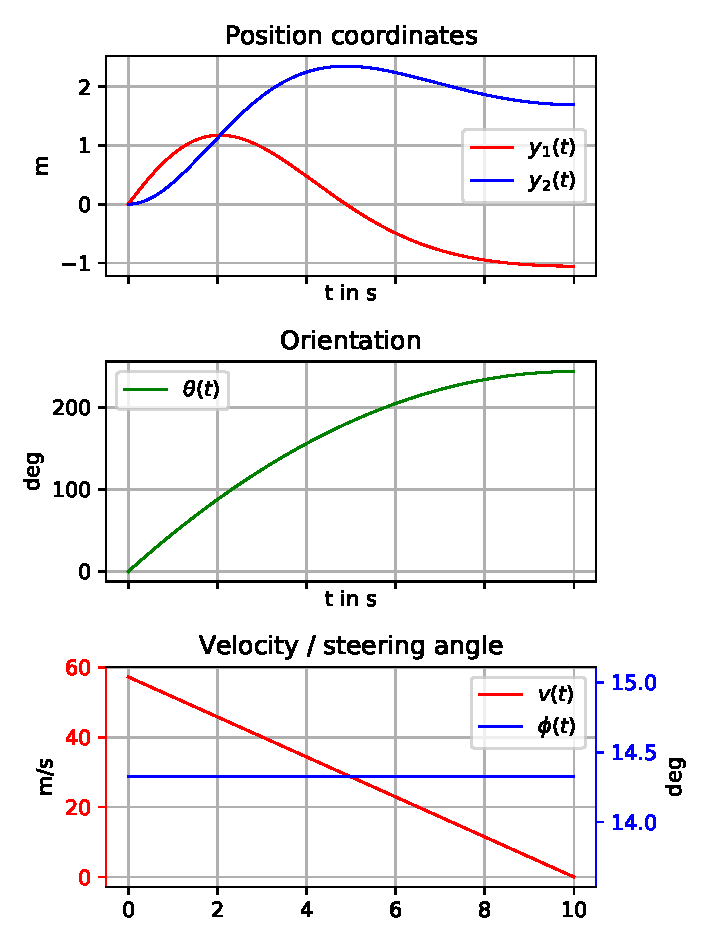
\includegraphics[width=0.7\textwidth]{img/state_trajectory.pdf}      
 \caption{State and control trajectory plot created with \mpl.}
 \label{fig:Test}
\end{figure} 


\FloatBarrier

\section{Animation using \mpl} \label{sec:animation}

\textbf{\py source code file: \texttt{02\_car\_example\_animation.py}}

Plotting the state trajectory is often sufficient, but sometimes it can be helpful to have a visiual represantation of the system to get a better understanding of what is actually happening. This applies especially for mechanical systems. \mpl provides the sub-package \emph{animation}, which can be used for such a purpose. We therefore need to add 
\listcodeanim{6}{6}
to the top of our code used in the previous sections. Under Windows it might be necessary to explicitely specify the path to the ffmpg library, e.g.:
\listcodeanim{7}{7}
FFMPG can be downloaded from \url{https://www.ffmpeg.org/download.html}.

We encapsulate all functions for the animation in a function called \texttt{car\_animation()}. At first we create a figure with two empty plots into which we will later draw the car and the curve of the trajectory dependung on the state \texttt{x}, the control input \texttt{u} and the parameters:
\listcodeanim{137}{165}
The handles \texttt{h\_x\_traj\_plot} and \texttt{h\_car} are used later to draw onto the axes.

During animation we want to display a representation of our car in this figure. We do this by plotting lines. All lines that represent the car are defined by points, which depend on the current state $\x$ and control signal $\uu$. This means we need to define a function inside \emph{car\_animation()} that maps from $\x$ and $\uu$ to a set of points in the $(Y_1,Y_2)$-plane using geometry and passes these to the plot instance \emph{car}:
\listcodeanim{167}{226}
Note that we are in the scope of the \texttt{car\_animation} function and have full acess to the handle \texttt{h\_car} here.

For the animation to work we need to define another two functions, \emph{init()} and \emph{animate(i)}. They will be later called by \mpl to initialize and perform the animation. The \emph{init()}-function defines which objects change during the animation, in our case the two axes the handles of which are returned:
\listcodeanim{225}{234}

The \emph{animate(i)}-function assigns data to the changing objects, in our case the car, trajectory plots and the simulation time (as part of the axis):
\listcodeanim{236}{250}

Finally we instanciate an object of \texttt{FuncAnimation} of the animation subpackage of \mpl. There, we pass the \texttt{animate} and \texttt{ini } to the constructor:
\listcodeanim{252}{258}

Note that all lines from 138 to 257 belong to the function \texttt{car\_animation}!

Now we have all things set up to simulate our system and animate it.
\listcodeanim{274}{277}

\begin{figure}[ht]
  \centering
  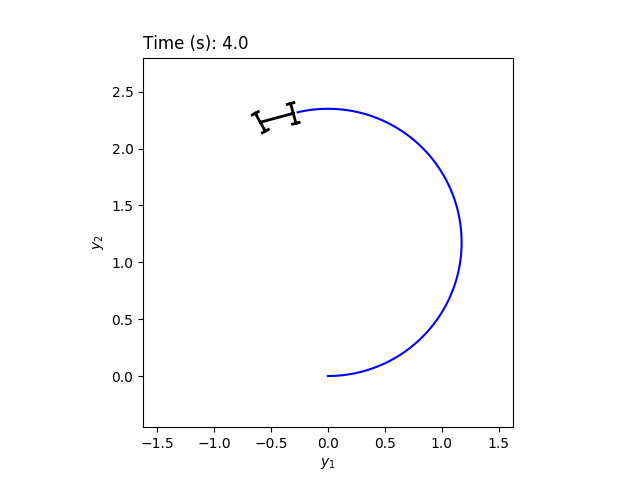
\includegraphics[width=0.7\textwidth]{img/animation}
  \caption{Car animation}
  \label{fig:animation}
\end{figure}
        



\section{Simulation with \scipy's new \emph{solve\_ivp} module and the \emph{lambda} function}\label{sec:ScipyLambda}

\textbf{\py source code file: \texttt{03\_car\_example\_scipy\_solve\_ivp.py}}

In addition to the solution in \autoref{sec:simulation} using \emph{odeint}, \scipy's integrate package contains some newer and more powerful solver functions. One of them is the function \href{https://docs.scipy.org/doc/scipy/reference/generated/scipy.integrate.solve_ivp.html}{\texttt{solve\_ivp}}. The function \texttt{solve\_ivp} takes a function of the type \texttt{func(t, x)} calculating the value of the right hand side of \eqref{eq:odesys}. Further parameters are not allowed. In order to be able to use our previously defined ode-function \texttt{ode(x, t, p)} which additionally takes the parameter structure \texttt{p} and has a different order for \texttt{t}  and \texttt{x}, we make use of a so-called lambda-function. We call the solver as follows:
\begin{lstlisting}
sol = solve_ivp(lambda t, x: ode(x, t, para), 
               (t0, tf), x0, method='RK45',t_eval=tt)
\end{lstlisting}
This way we encapsulate our \texttt{ode} function in an anonymous function, that has just $(t, x)$ as arguments (as required by \texttt{solve\_ivp}) but evaluates as \texttt{ode(x, t, para)}\footnote{The lambda function corresponds to @ in \emph{MATLAB}}. Additionally, the following arguments are passed to \texttt{solve\_ivp}: A tuple $(t0, tf)$ which defines the simulation interval and the initial value $x0$. Furthermore, we pass the optional arguments \emph{method}, in this case a Runge-Kutta method and \emph{t\_eval}, which defines the values at which the solution should be sampled.

The return value \emph{sol} is an \emph{OdeResult} object. To extract the simulated state trajectory, we execute:
\begin{lstlisting}
x_traj = sol.y.T # size=len(x)*len(tt) (.T -> transpose)
\end{lstlisting}


\printglossaries
\end{document}

%%% Local Variables:
%%% mode: latex
%%% TeX-master: t
%%% End: